\documentclass{article}

\usepackage{arxiv}

\usepackage[utf8]{inputenc} % allow utf-8 input
\usepackage[T1]{fontenc}    % use 8-bit T1 fonts
\usepackage{hyperref}       % hyperlinks
\usepackage{url}            % simple URL typesetting
\usepackage{booktabs}       % professional-quality tables
\usepackage{amsfonts}       % blackboard math symbols
\usepackage{nicefrac}       % compact symbols for 1/2, etc.
\usepackage{microtype}      % microtypography
\usepackage{lipsum}         % Can be removed after putting your text content
\usepackage{graphicx}
\usepackage[authoryear]{natbib}
\usepackage{doi}
\usepackage{amssymb,amsmath,latexsym,amsthm,amsfonts,bbm,dsfont}
\usepackage{bbold}
\usepackage{cleveref}       % smart cross-referencing

\setcounter{MaxMatrixCols}{20}

\newcommand{\bigzero}{\mbox{\normalfont\Large\bfseries 0}}
\newcommand{\rvline}{\hspace*{-\arraycolsep}\vline\hspace*{-\arraycolsep}}



\newcommand{\PP}{\mathcal{P}}
\newcommand{\pp}{\mathbf{p}}
\newcommand{\p}{\mathds{P}}
\newcommand{\E}{\mathds{E}}
\newcommand{\V}{\mathds{V}}
\newcommand{\vv}{\mathbf{v}}
\newcommand{\C}{\mathcal{C}}
\newcommand{\D}{\mathcal{D}}
\newcommand{\e}{\mathbf{e}}

\title{Approximating convergence time of Stackelberg-Nash based ratio via Markov Chain Absorption Times}

% Here you can change the date presented in the paper title
\date{June 30, 2025}
% Or remove it
%\date{}

\author{ \href{https://orcid.org/0000-0000-0000-0000}{
\includegraphics[scale=0.06]{orcid.pdf}\hspace{1mm} Nicolas I. Boyardi Alache}\\
	Department of Industrial Engineering\\
	Universidad Técnico Federico Santa María\\
	Valparaíso, Chile\\
	\texttt{nicolas.boyardi@usm.cl} \\
	%% examples of more authors
	%% \AND
	%% Coauthor \\
	%% Affiliation \\
	%% Address \\
	%% \texttt{email} \\
	%% \And
	%% Coauthor \\
	%% Affiliation \\
	%% Address \\
	%% \texttt{email} \\
	%% \And
	%% Coauthor \\
	%% Affiliation \\
	%% Address \\
	%% \texttt{email} \\
}

% Uncomment to override  the `A preprint' in the header
%\renewcommand{\headeright}{Technical Report}
%\renewcommand{\undertitle}{Technical Report}
\renewcommand{\shorttitle}{Stackelberg-Nash Markov Chain time stimation}

%%% Add PDF metadata to help others organize their library
%%% Once the PDF is generated, you can check the metadata with
%%% $ pdfinfo template.pdf
\hypersetup{
pdftitle={A template for the arxiv style},
pdfauthor={Nicolás I. Boyardi Alache},
pdfkeywords={Markov Chain, Stackelberg games, Nash Equilibrium},
}

\begin{document}
\maketitle

\begin{abstract}
	In Game Theory, more precisely in Security Games, Stackelberg Games are used to represent problems involving 2 or more actors under a hierarchical relationship between them. This setting is useful to, in particular, model the problem (from the perspective of an authority) of evasion in public transport systems \citep{FareInspection} \citep{BROTCORNE20211}.\par
In the aforementioned papers it is discussed thoroughly the necessity of the operational implementation of the probabilities of inspection in public transportation systems, obtained by solving a multi-level optimization problem. This problem solves simultaneously the minimization of the evasion and the minimization of risk of the opportunistic passengers in being inspected.\par
In particular, it is of interest to know how much time (days) it will take to the evasion rate to converge to the one obtained through the steady-state probabilities obtained during optimization. Monte Carlo simulations were done in order to estimate this time in the papers cited previously. This approach has a latent problem. There is no \textit{a priori} knowledge of how much time the simulation has to run in order to converge. So, in not-so-rare cases it could take more than one year time in instances, making this evasion rate both useless (as this needs to be implemented in mid term) and expensive, because these simulations are costly.\par
This work aims to establish a second method to obtain the time it should take the evasion rate converge to the theoretical steady-state one via Markov Chains. Specifically, this work seeks to construct a Markov Chain that permits to deduce, or approximate, this convergence time.\par
%
\end{abstract}


% keywords can be removed
\keywords{Markov Chain, Stackelberg games, Nash Equilibrium}

\section{Introduction}
In Game Theory, more precisely in Security Games, Stackelberg Games are used to represent problems involving 2 or more actors under a hierarchical relationship between them. For example, but not limited to, it let us model the problem of evasion in public transport systems from the perspective of the transit authority \citep{FareInspection} \citep{BROTCORNE20211}. Another example is the work of \citep{Carrasco}, where a Stackelberg-Nash problem, which model the problem of street vending in the city of Valparaiso, Chile, is addressed. In any case, the operational implementation of the solution of the optimization problem rests on the construction of daily inspection schedules, which, in the long run, decreases the evasion rate (ER) or the Illegal Occupation Rate (IOR), respectively. Both the ER and the IOR represents the fraction of actors under an undesirable behavior (Percentage of persons evading paying the public transport tariff or of persons selling in the streets). Since there is limited resources to inspect, this daily schedules have to be implemented randomly daily for some time before it induces change in behavior. In that sense, it matters how fast this convergence occurs. To estimate that, Monte Carlo simulations were carried out, measuring the mean time it takes to have a daily ER or IOR less than some threshold.\par
The present work aims to estimate the convergence time to the equilibrium IOR via Markov Chain absorption times. Here, a Markov chain is built around the Nash-Equilibrium density distribution of actors $\pp^*$, obtained through the optimal solution of the Stackelberg-Nash Problem. The chain replicates the behavior near the Nash Equilibrium, as the like of an harmonic oscillator.\par 
This work is organized as follows. A brief resume on how the Nash Equilibrium is built is in \autoref{sec2}. \autoref{sec3} formulates a Markov Chain that approximates the dynamic of the Stackelberg-Nash game. \autoref{sec4} presents some actual computations based on the theory built in \autoref{sec3}. Finally, in \autoref{sec5} concludes this work presenting some conclusions and advice for future work.\par


\section{The Stackelberg-Nash model}\label{sec2}
In this section will be discussed briefly where does the probabilities, that are used as parameters for the model in this work, came from. The model Stackelberg-Nash model discussed in the next section is a one-to-one replica of the one from \citep{Carrasco}, where the setting is the management of street vending in the city of Valparaíso, Chile. The understanding of the variables, that will be parameters later, involved in the Nash Equilibrium Problem is important for this work.\par

From that, let $J$ be the set of sites where an action could take place (e.g. street vending). It is defined a subset $L \subsetneq J$ of authorized\footnote{Legal in the context of street vending, thus the capital $L$.} sites where the action is acceptable to occur, and $I\subsetneq J$ the subset of unauthorized sites where it is not acceptable. Obviously, $I \cap L = \emptyset$ and $I \cup L = L$. The attractiveness of a site $j \in J$ is defined by the parameter $B_j$, such that $\min_{i \in I} B_i > \max_{l \in L} B_l$. That is, the worst attractive unauthorized site is more attractive than the best authorized site. In terms of street vending it makes sense, because usually unauthorized places are cheaper because of lack of rental of place, flexibility, etc.\par
Let $m$ be the number of actors acting over $J$. The distribution of the actors over the $J$ sites is represented by the vector $\pp = (p_j)_{j\in J} \in \mathbb{R}^{|J|}$, such that $\mathbb{1}_{|J|}^\top\pp = 1$ and $\pp \geq \mathbb{0}_{|J|}$.\par
The objective of an authority is to thwart the actions of the subjects over unauthorized sites $I$. To do so, the authority counts with a small set of $n$ teams that induce aversion in the total attractiveness of a site. Let $\p_j$ be the probability of an intervesion ocurring in site $j \in J$, with a aversion of $\overline{W} \in \mathbb{R}$. In the same line, a total-atractiveness function $U(p_j \vert B_j, \p_j)$ is defined for every site $j \in J$. This function is strictly increasing in $B_j$; non-increasing in $p_j$, measuring the saturation on a spatial sense; and non-increasing in aversion, as higher probabilities of being inspectioned implies lower expected utility.\par
The Nash Equilibrium Problem that finds the distribution $\pp$ of actors, given the aversion probabilities $\p \in \mathds{R}^{|J|}$, such that this is configuration is a Nash Equilibrium, is defined by (\citep{Carrasco}):
\begin{align*}
	NE(\p) :  \;\; p_j(\gamma -B_j U(p_j\vert B_j, \p_j)(1-\p_j) - \overline{W}\p_j) &= 0 & \forall j \in J\\
	B_j U(p_j\vert B_j, \p_j)(1-\p_j) - \overline{W}\p_j &\leq \gamma& \forall j \in J\\
	\mathbb{1}^{\top}_{|J|}\p  &= 1&\\
	\pp &\geq \mathbb{0}_{|J|}& \\
\end{align*} 
The problem of finding optimal aversion probabilities $\p^*$ is discussed thoroughly in the aforementioned work of street vending. That discusion is out of the scope of this work, because both $\p^*$ and $\pp^*$ will be treated as parameters.\par

\section{The Markov Model}\label{sec3}
After doing the corresponding optimizations, it stays open the practical implementation of intervention teams given the aversion probabilities obtained. In \citep{Carrasco}, they interpreted probabilities of intervention as frequency, that is, the fraction of the days from a given time horizon that a given place must be inspected during those days. In addition, given the optimal Illegal Occupation Rate (IOR) $Ior^* := \sum\limits_{i \in I} p^*_i$, they asked how much time, considering a day-by-day implementation of the aversion probabilities, it will take to the actors drop the daily IOR $Ior(t)$ to the optimal.\par
The only approach in said work was to do Monte-Carlo Simulation. The setting considered counting the fraction of time, until that day, that a given site has been intervened as the aversion probabilities. The probability of selecting a site $j$ is given by the optimal $\p^*_j$. By the Law of Large Numbers, this setting guarantees that $Ior(t) \rightarrow Ior^*$ as $t\rightarrow \infty$. So, day by day, they solved the Nash Equilibrium Problem $NE(t)$ with the aversion probabilities obtained by the Montecarlo simulation. After that, they computed the actual IOR, $Ior(t)$, and obtained the convergence time as the first arrival under the optimal IOR $Ior^*$. That is, $\tau = \min \{t \;\vert\; Ior(t) < Ior^*\}$ is the time they considered has to pass until a day-by-day implementation of the aversion probabilities makes the actors converge to the Nash Equilibrium, in the IOR sense.\par
In this section, an alternative method will be described to obtain the convergence time of the IOR, $\tau$.\par
Let $\{X(j)_t\}_{t=\in \mathbb{N}, j \in J}$ be a Markov chain that represents the proportion of actors for every site $j$ at time $t$. So, $m\cdot X(j)_t \in \{0,1 \dots m\}$ is the quantity of actors in $j$ at $t$. It is assumed that for fixed $j$, $\{X(j)_{t}\}_{t=0}^m$ is a Markov Chain on its own. For any two $j \not= j^{'} \in J$, the Markov Chains defined are independently one to another.\par

\subsection{Transition Matrix}
In this section, the construction of the transition matrix is addressed.
Let $P \in \mathbb{R}^{(m+1+|J|)^2}$ be the transition matrix of the Markov Chain $\{X(j)_t\}_{t \in \mathds{N}, j \in J}$. As the Markov Chain measures quantity (and does not model individually every actor), it is assumed that $P$ is a block-diagonal matrix, having $|J|$ diagonal blocks $P(j) \in \mathbb{R}^{(m+1)^2}$:\par
\begin{align*}
	P =
	\left( \begin{array}{@{}c|@{}c|@{}c|c@{}}
		P(j_1) & \mathbb{0} & \dots & \mathbb{0}\\
		\hline
		\mathbb{0} & P(j_2) & \dots & \mathbb{0}\\
		\hline
		\vdots & \vdots & \ddots & \vdots\\
		\hline
		\mathbb{0} & \mathbb{0} & \dots & P(j_{|J|})\\
	\end{array}	\right).
\end{align*}
Now, let $j \in J$ be fixed. To replicate the behavior, from the perspective of Game Theory, of the Nash Equilibrium, the probabilities will be distributed according to the distance of the actual proportion to the optimal $p^*_j$. That is, if the distribution of proportions is distant from the optimal, then the former carries momentum towards the optimal distribution. For sake of simplicity, the relationship between a given actual proportion and the optimal is considered to be linear and symmetrical.\par
Let $a,b \in \{0,\frac{1}{m} \dots 1\}$, $\Delta_a := |p^*_j - a|$ and $[p^*_j] := \lceil m\cdot p^*_j\rfloor/m$, where $\lceil\cdot \rfloor$ is the nearest-integer function. So, we have that the transition probabilities from $a$ to $b$ is:
\begin{align*}
	P(j)_{ab} := \begin{cases}
		C_{a,1}(C_{a,2} - |p^*_j - b|), & \text{if } a \not = [p^*_j] \text{ and } |p^*_j - b| < \Delta_a,\\
		1 & \text{if } a = b = [p^*_j],\\
		0 & \text{in other case},
	\end{cases}
\end{align*}
where $C_{a,1}$ and $C_{a,2}$ are constants ensuring 2 properties: that this is, in fact, a discrete distribution, and that nulls out for any $b$ such that $|p^*_j - b| \geq \Delta_A$. Following the definition, for $a \not= [p^*_j]$, then $b = a$ is the nearest point to $p^*_j$ outside the support of $P(j)_{a \cdot}$. So:\par
\begin{align*}
	P(j)_{aa} = C_{a,1}(C_{a,2} - \Delta_a) = 0 \implies C_{a,2} = \Delta_a.
\end{align*}
On the other hand, for every $a$, $P(j)_{a \cdot}$ is a probability distribution, so it has to sum exactly to $1$ over all the values of $b \in \{0,\frac{1}{m} \dots 1\}$. If we define $s^-_{a,j} := \lceil m(p^*_j - \Delta_a) \rceil$ and $s^+_{a,j} := \lfloor m(p^*_j + \Delta_a) \rfloor$, then the condition $|p^*_j - b| < \Delta_a$ is equivalent to $m\cdot b \in \left\{s^-_{a,j} , \dots, s^+_{a,j}\right\} \subset \mathds{N}$. So, we have that:
\begin{align*}
	\sum\limits_{k = 0}^{m} P(j)_{a\frac{k}{m}} &= 1.\\
	\Longleftrightarrow \sum\limits_{k = s^{-}_{a,j}}^{s^{+}_{a,j}} C_{a,1}(\Delta_a -|p^*_j-k/m|) &= 1.\\
	\Longleftrightarrow C_{a,1} &= \bigg(\sum\limits_{k = s^-_{a,j}}^{s^+_{a,j}} (\Delta_a -|p^*_j-k/m|)\bigg)^{-1}.\\
\end{align*}

For example, for some $j_1 \in J$, $m = 10$, $p_{j_1}^* = 5.3$, the $j_1$-th transition matrix $P(j_1)$ is:
\begin{align*}
	\begin{pmatrix}
		0     & 0.036 & 0.071 & 0.107 & 0.143 & 0.179 & 0.164 & 0.129 & 0.093 & 0.057 & 0.021 \\
		0     & 0     & 0.054 & 0.109 & 0.163 & 0.217 & 0.196 & 0.141 & 0.087 & 0.033 & 0     \\
		0     & 0     & 0     & 0.093 & 0.185 & 0.278 & 0.241 & 0.148 & 0.056 & 0     & 0     \\
		0     & 0     & 0     & 0     & 0.192 & 0.385 & 0.308 & 0.115 & 0     & 0     & 0     \\
		0     & 0     & 0     & 0     & 0     & 0.625 & 0.375 & 0     & 0     & 0     & 0     \\
		0     & 0     & 0     & 0     & 0     & 1     & 0     & 0     & 0     & 0     & 0     \\
		0     & 0     & 0     & 0     & 0     & 1     & 0     & 0     & 0     & 0     & 0     \\
		0     & 0     & 0     & 0     & 0.143 & 0.5   & 0.357 & 0     & 0     & 0     & 0     \\
		0     & 0     & 0     & 0.056 & 0.194 & 0.333 & 0.278 & 0.139 & 0     & 0     & 0     \\
		0     & 0     & 0.029 & 0.103 & 0.176 & 0.25  & 0.221 & 0.147 & 0.074 & 0     & 0     \\
		0     & 0.018 & 0.064 & 0.109 & 0.155 & 0.2   & 0.182 & 0.136 & 0.091 & 0.045 & 0
	\end{pmatrix}.
\end{align*}
Likewise, for $j_2 \in J$, with $p^*_{j_2} = 7.8$, the matrix $P(j_2)$ is:
\begin{align*}
	\begin{pmatrix}
		0     & 0.021 & 0.042 & 0.063 & 0.084 & 0.105 & 0.126 & 0.146 & 0.159 & 0.138 & 0.117 \\
		0     & 0     & 0.026 & 0.053 & 0.079 & 0.106 & 0.132 & 0.159 & 0.175 & 0.148 & 0.122 \\
		0     & 0     & 0     & 0.035 & 0.069 & 0.104 & 0.139 & 0.174 & 0.194 & 0.160 & 0.125 \\
		0     & 0     & 0     & 0     & 0.048 & 0.096 & 0.144 & 0.192 & 0.221 & 0.173 & 0.125 \\
		0     & 0     & 0     & 0     & 0     & 0.072 & 0.145 & 0.217 & 0.261 & 0.188 & 0.116 \\
		0     & 0     & 0     & 0     & 0     & 0     & 0.128 & 0.256 & 0.333 & 0.205 & 0.077 \\
		0     & 0     & 0     & 0     & 0     & 0     & 0     & 0.313 & 0.500 & 0.187 & 0     \\
		0     & 0     & 0     & 0     & 0     & 0     & 0     & 0     & 1     & 0     & 0     \\
		0     & 0     & 0     & 0     & 0     & 0     & 0     & 0     & 1     & 0     & 0     \\
		0     & 0     & 0     & 0     & 0     & 0     & 0     & 0.286 & 0.714 & 0     & 0     \\
		0     & 0     & 0     & 0     & 0     & 0     & 0.083 & 0.292 & 0.417 & 0.208 & 0
	\end{pmatrix}
\end{align*}
The graph of $P(j_1)_{ab}$ is shown as a function of $b$ in figure \ref{fig:function}.\par

\begin{figure}[h!]
    \centering
    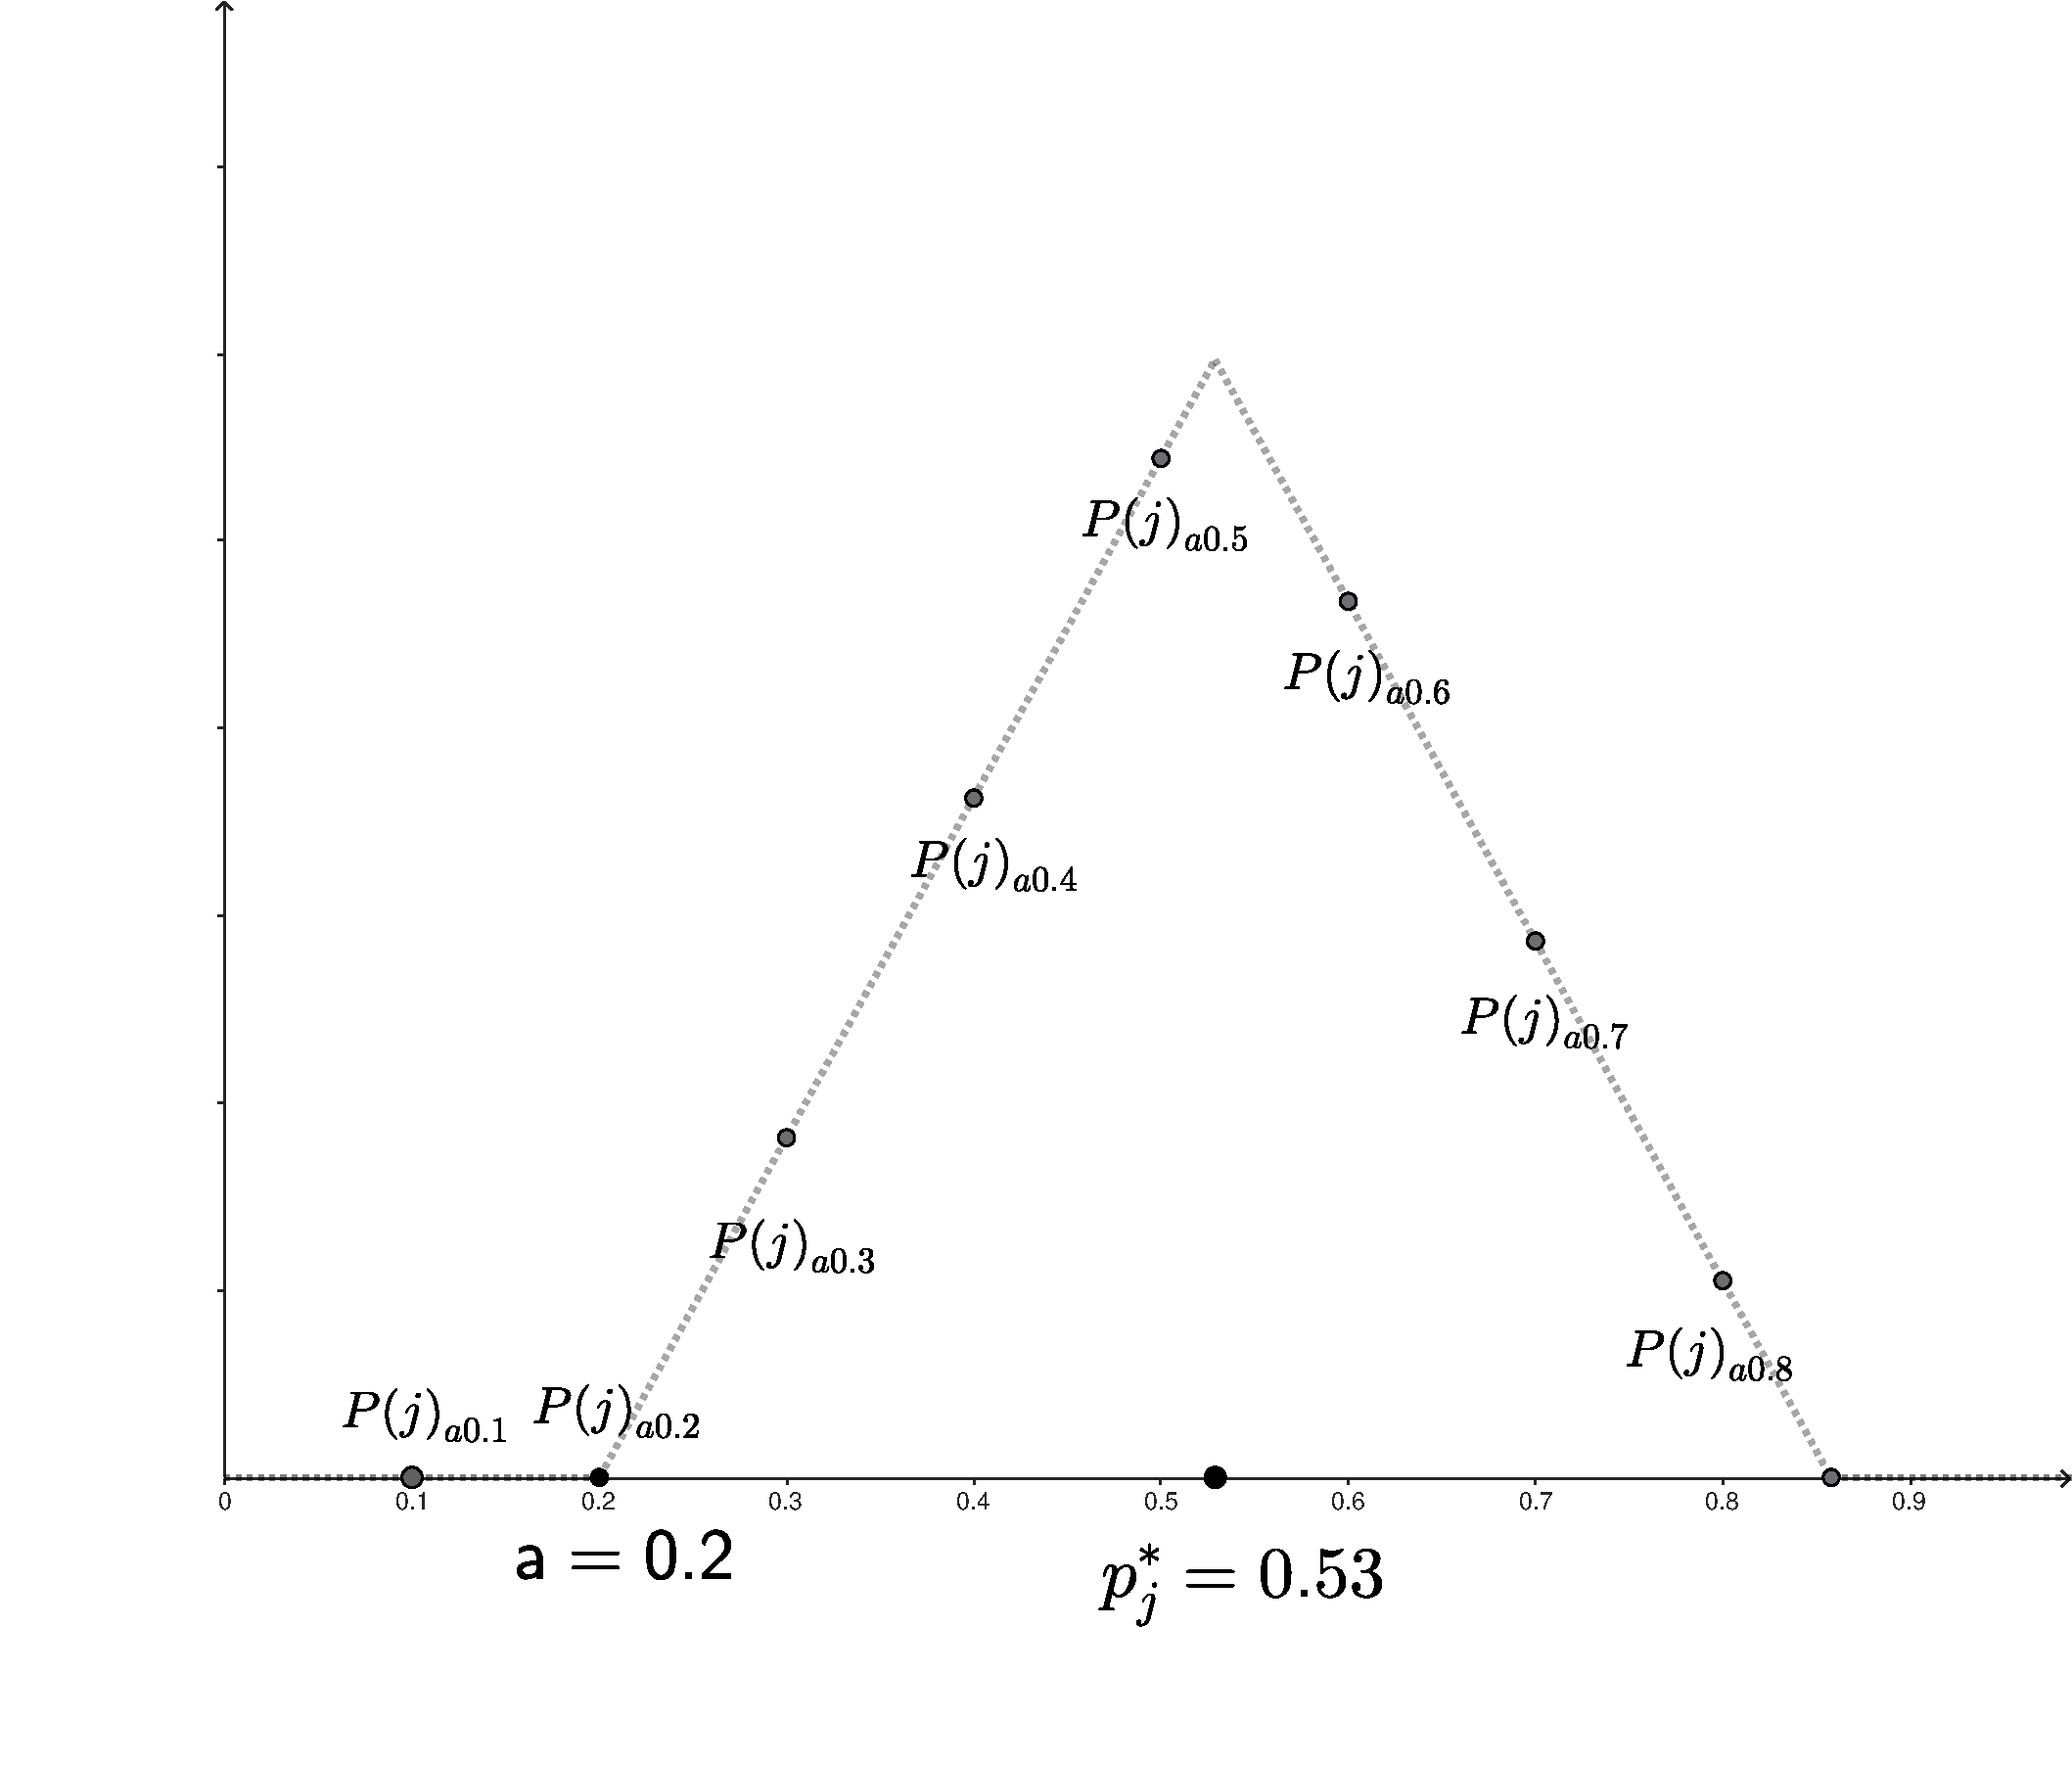
\includegraphics[width = 14 cm]{img/geogebra-export (5).pdf}
    \caption{Example of the conditional probabilities $P(j)_{ab}$, for fixed $j$, $a$, $p^*_j$ and for $b \in \{0.1, 0.2, 0.3, 0.4, 0.5, 0.6, 0.7, 0.8\}$. The dotted lines shows the continuous interpolator of the conditional probabilities.}
	\label{fig:function}
\end{figure} 

\subsection*{Absorption times and convergence}
It is easy to see that every transition matrix in the diagonal of $P$, $P(j)$, has an absorbing class of at most 2 elements. The absorbing class usually consists of the nearest element in the lattice $\{0,\frac{1}{m}, \dots, 1\}$ to $p^*_j$, or the 2 nearest elements, if it turns out to be the case (because of roundings, numerical errors, etc.).\par
So, with respect to $P$, it is easy to see that after reordering its entries according to the canonical form the matrix $Q$ of $P$ is given in terms of the matrices $Q(j)$ of each $j$-th Markov Chain in the diagonal of $P$:

\begin{align*}
	Q =
	\left( \begin{array}{@{}c|@{}c|@{}c|c@{}}
		Q(j_1) & \mathbb{0} & \dots & \mathbb{0}\\
		\hline
		\mathbb{0} & Q(j_2) & \dots & \mathbb{0}\\
		\hline
		\vdots & \vdots & \ddots & \vdots\\
		\hline
		\mathbb{0} & \mathbb{0} & \dots & Q(j_{|J|})\\
	\end{array}	\right).
\end{align*}
Once more, due to the diagonal structure of $P$, the fundamental matrix of $P$, $F$, is obtained as the diagonal matrix containing in its $j$-th diagonal block the matrix $F(j)$, where
\begin{align*}
	F(j) := (Id - Q(j))^{-1},
\end{align*}
that is
\begin{align*}
	F =
	\left( \begin{array}{@{}c|@{}c|@{}c|c@{}}
		F(j_1) & \mathbb{0} & \dots & \mathbb{0}\\
		\hline
		\mathbb{0} & F(j_2) & \dots & \mathbb{0}\\
		\hline
		\vdots & \vdots & \ddots & \vdots\\
		\hline
		\mathbb{0} & \mathbb{0} & \dots & F(j_{|J|})\\
	\end{array}	\right)
\end{align*}
It is known that the absorption time, starting from a transient state $a$ is given by the formula
\begin{align*}
	\e_{ma}^{\top} F\mathbb{1}_l
\end{align*}
where $\e_{ma}$ is the $ma$-th element of the canonical base of $\mathbb{R}^l$, for a addecuate constant $l \in \mathds{N}$ (remember that $ma \in \{0, 1, \dots , m\}$). Moreover, the expected absorption time, as the mean over all posible initial states, is given by:
\begin{align*}
	\tau := \frac{\mathbb{1}_l^{\top}F \mathbb{1}_l}{l}.
\end{align*}
Again, by the diagonality of $P$, this expected time reduces to:
\begin{align*}
	\tau = \frac{\sum_{j \in J}\mathbb{1}_{l(j)}^{\top}F(j) \mathbb{1}_{l(j)}}{l},
\end{align*}
where $l(j)$ is equal to the quantity of transient states of the $j$-th Markov Chain, that is, $m+1 - Abs(j)$. So, $l = \sum\limits_{j \in J} l(j) = (m+1)|J|- Abs$, where $Abs = \sum\limits_{j \in J} Abs(j)$ is the total quantity of absorbing states over $P$.\par

\subsection{Illegal Occupation rate}
Now everything is available to compute the IOR with respect to the absorbing time $\tau$. Assuming that the initial distribution of actors across the $|J|$ sites is uniformly distributed, observe that:
\begin{align*}
	Ior(\tau) 	&= \E\left(\sum\limits_{i \in I} X(i)_{\lceil \tau \rfloor}\right),\\
				&= \sum\limits_{i \in I} \E(X(i)_{\lceil \tau \rfloor}),\\
				&= \sum\limits_{i \in I} \sum\limits_{b} \p(X(i)_{\lceil \tau \rfloor} = b)\cdot b,\\
				&= \sum\limits_{i \in I} \sum\limits_{b}\sum\limits_{a} \underbrace{\p(X(i)_{\lceil \tau \rfloor} = b \; \vert \;\;X(i)_{0} = a)}_{ = P^{{\lceil \tau \rfloor}}_{ab}(i)} \cdot \p(X(i)_0 = a)\cdot b,\\
				&= \sum\limits_{i \in I} \sum\limits_{a}\sum\limits_{b} \frac{1}{m+1}P^{{\lceil \tau \rfloor}}_{ab}(i)\cdot b,\\
				&= \sum\limits_{i \in I} \frac{\mathbb{1}_{|I|}^{\top}P^{{\lceil \tau \rfloor}}(i)\vv}{m+1},\\
\end{align*}
where $\vv = (0, 1, \dots, m)/m \in \mathds{R}^{m+1}$.\par

\section{Numerical Experiments}\label{sec4}
The data set used in this work is the same as in \citep{Carrasco}. That is the common parameters $m = 974$, $|I| = 102$ and $|L| = 40$ and the varying parameter $n \in\{1, 2 \dots 15\}$ and the optimal probabilities $\pp^*(n)$.\par
Following the author's analysis, lets fix $n=10$. One can compute the equilibrium IOR, obtaining that $Ior^* \approx 0.47681$. Then, both $\tau$ and $Ior(\tau)$ are computed, obtaining $\tau \approx 4.67541$ and $Ior(\tau) \approx 0.60012$. Considering $\tau+1$ instead, the IOR improves dramatically, to $Ior(\tau+1) \approx = 0.50752$. This may seem artificial, but serves as a compensation for the  oversimplification of considering $P$ block-diagonal, which holds accurate only near the equilibrium.\par
Further experiments show that for $t < \tau$, one may obtain unrealistic values for IOR, such as $Ior(1) \approx 16$, or $Ior(2) \approx 5$. As a ratio, this number should always be not greater than $1$, but in the early stages of the iterations this could easily not be the case because some high-density cases for every site $j$ might occur at the same time.\par
It is worth mentioning that for $t \gtrapprox 2\tau$, $Ior(t) \approx Ior^*$. So the transition matrix, at least in a limiting case, works as intended (the Markov IOR converges to the equilibrium one).\par
Now, the same experiments were carried out for every $n \{ 1,2 \dots 15\}$. The results are shown in \ref{fig:tau_n} and \ref{fig:Ior_tau_n}.\par

\begin{figure}
	\centering
	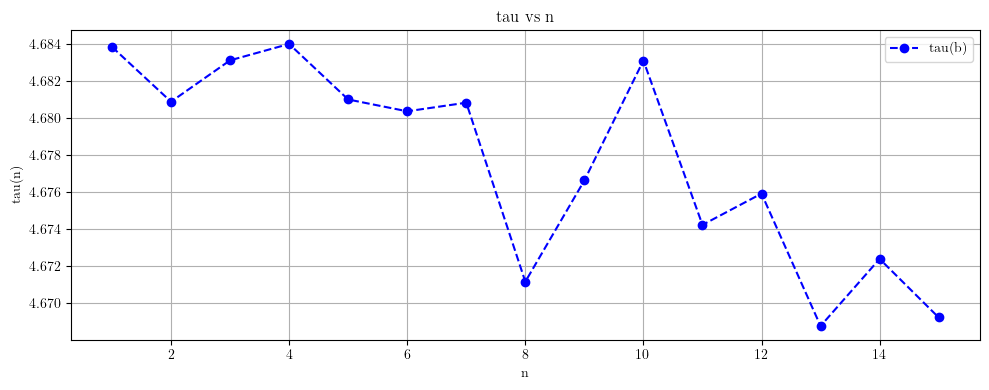
\includegraphics[width = 0.9 \textwidth]{img/tau_n.png}
	\caption{Plot of $\tau(n)$, for $n \in \{1, 2 \dots 15\}$.}
	\label{fig:tau_n}
\end{figure}
\begin{figure}
	\centering
	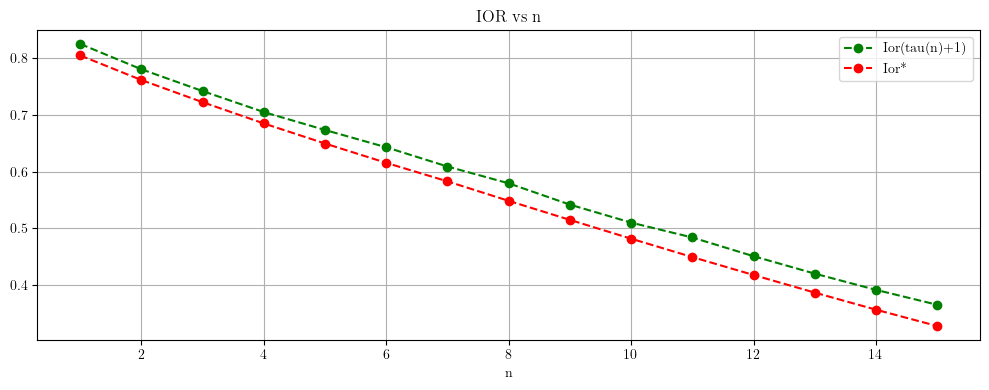
\includegraphics[width = 0.9 \textwidth]{img/Ior_tau_n.png}
	\caption{Plot of $Ior(\tau(n)+1)$, for $n \in \{1, 2 \dots 15\}$(green) and $Ior^*(n)$ (red), for reference.}
	\label{fig:Ior_tau_n}
\end{figure}

From here, the analysis does not change essentially as $n$ changes, i.e., the Markov Chain converges rapidly towards the Nash Equilibrium.\par
As reported in \cite{Carrasco}, for $n=10$ it is expected that after $58$ days the IOR hits the threshold of $52\%$ for the first time. This value is vastly greater than the theoretical $\approx 48\%$. This value is the best that the authorities expect to reduce the IOR, so it stays as the threshold for which any solution that achieves this value, or lesser, is considered a good solution. For other values of $n$ there has not been an extensive analysis, so it has been left out in this work aswell.\par

\section{Conclusions}\label{sec5}
It is clear that the Markov Model proposed has a very rapid convergence compared to the Montecarlo simulations. This may be due to the fact that the transition matrix $P$ is built very naively. Intuitively, the graph of a set of states approaching a Nash Equilibrium should look like an spring, i.e., said states should look like they are revolving around the equilibrium. That may not be the case for the way the transition matrix was built in this work, because it puts major weight towards the equilibrium, but does not address the fact that the momentum of a given state before absorption may induce higher probabilities to not converge immediately, if it is not near the equilibrium. Coming back to the spring comparison, an spring that is set off farther from its equilibrium will oscillate further. On other side, the analysis is still reasonable, as the IOR converges accordingly.\par
Improvements would come from a better modeling of the transition matrix, as described in the last paragraph.\par 

\section*{Code}
The Python programmes used in the computations of this work are up in \href{https://github.com/NeutralElement/Stochastic-Processes-Project}{this github repository}.

\newpage
\bibliographystyle{unsrtnat}
\bibliography{bibliografia}  %%% Uncomment this line and comment out the ``thebibliography'' section below to use the external .bib file (using bibtex) .


%%% Uncomment this section and comment out the \bibliography{references} line above to use inline references.
% \begin{thebibliography}{1}

% 	\bibitem{kour2014real}
% 	George Kour and Raid Saabne.
% 	\newblock Real-time segmentation of on-line handwritten arabic script.
% 	\newblock In {\em Frontiers in Handwriting Recognition (ICFHR), 2014 14th
% 			International Conference on}, pages 417--422. IEEE, 2014.

% 	\bibitem{kour2014fast}
% 	George Kour and Raid Saabne.
% 	\newblock Fast classification of handwritten on-line arabic characters.
% 	\newblock In {\em Soft Computing and Pattern Recognition (SoCPaR), 2014 6th
% 			International Conference of}, pages 312--318. IEEE, 2014.

% 	\bibitem{hadash2018estimate}
% 	Guy Hadash, Einat Kermany, Boaz Carmeli, Ofer Lavi, George Kour, and Alon
% 	Jacovi.
% 	\newblock Estimate and replace: A novel approach to integrating deep neural
% 	networks with existing applications.
% 	\newblock {\em arXiv preprint arXiv:1804.09028}, 2018.

% \end{thebibliography}


\end{document}
